 %----------------------------------------------------------------------------------------
%	PACKAGES AND OTHER DOCUMENT CONFIGURATIONS
%----------------------------------------------------------------------------------------

\documentclass[12pt]{scrartcl} % Font size

%----------------------------------------------------------------------------------------
%	PACKAGES AND OTHER DOCUMENT CONFIGURATIONS
%----------------------------------------------------------------------------------------

\usepackage{amsmath, amsfonts, amsthm} % Math packages

\usepackage{listings} % Code listings, with syntax highlighting

\usepackage[ngerman]{babel} % german language hyphenation

 \usepackage{setspace}

\usepackage[backend=biber, style=numeric-verb]{biblatex}
\addbibresource{literatur.bib}

\usepackage{graphicx} % Required for inserting images
\graphicspath{{Figures/}{./}} % Specifies where to look for included images (trailing slash required)

\usepackage{booktabs} % Required for better horizontal rules in tables

\numberwithin{equation}{section} % Number equations within sections (i.e. 1.1, 1.2, 2.1, 2.2 instead of 1, 2, 3, 4)
\numberwithin{figure}{section} % Number figures within sections (i.e. 1.1, 1.2, 2.1, 2.2 instead of 1, 2, 3, 4)
\numberwithin{table}{section} % Number tables within sections (i.e. 1.1, 1.2, 2.1, 2.2 instead of 1, 2, 3, 4)

\setlength\parindent{0pt} % Removes all indentation from paragraphs

\usepackage{enumitem} % Required for list customisation
\setlist{noitemsep} % No spacing between list items

%----------------------------------------------------------------------------------------
%	DOCUMENT MARGINS
%----------------------------------------------------------------------------------------

\usepackage{geometry} % Required for adjusting page dimensions and margins

\geometry{
	paper=a4paper, % Paper size, change to letterpaper for US letter size
	top=2.5cm, % Top margin
	bottom=3cm, % Bottom margin
	left=2.5cm, % Left margin
	right=2.5cm, % Right margin
	headheight=0.75cm, % Header height
	footskip=1.5cm, % Space from the bottom margin to the baseline of the footer
	headsep=0.75cm, % Space from the top margin to the baseline of the header
	%showframe, % Uncomment to show how the type block is set on the page
}

%----------------------------------------------------------------------------------------
%	FONTS
%----------------------------------------------------------------------------------------

\usepackage[utf8]{inputenc} % Required for inputting international characters
\usepackage[T1]{fontenc} % Use 8-bit encoding
\usepackage{textgreek}

\usepackage{mathptmx}
%\usepackage{fourier} % Use the Adobe Utopia font for the document

%----------------------------------------------------------------------------------------
%	SECTION TITLES
%----------------------------------------------------------------------------------------

\usepackage{sectsty} % Allows customising section commands

\sectionfont{\vspace{6pt}\centering\normalfont\scshape} % \section{} styling
\subsectionfont{\normalfont\bfseries} % \subsection{} styling
\subsubsectionfont{\normalfont\itshape} % \subsubsection{} styling
\paragraphfont{\normalfont\scshape} % \paragraph{} styling

%----------------------------------------------------------------------------------------
%	HEADERS AND FOOTERS
%----------------------------------------------------------------------------------------

\usepackage{scrlayer-scrpage} % Required for customising headers and footers

\ohead*{} % Right header
\ihead*{} % Left header
\chead*{} % Centre header

\ofoot*{} % Right footer
\ifoot*{} % Left footer
\cfoot*{\pagemark} % Centre footer
 % Include the file specifying the document structure and custom commands

%----------------------------------------------------------------------------------------
%	TITLE SECTION
%----------------------------------------------------------------------------------------

\title{	
	\normalfont\normalsize
	\textsc{Valentin-Heider-Gymnasium Lindau}\\
	\vspace{10pt}
	\textsc{Qualifikationsstufe Jahrgang 2021/23}\\
	\vspace{10pt}
	\begin{figure}[h] % [h] forces the figure to be output where it is defined in the code (it suppresses floating)
	\centering
	
\includegraphics[width=0.5\columnwidth]{VHGLogo.jpg} 
	\end{figure}
	
	\large\textsc
	W-Seminararbeit\\
	aus dem Fach\\
	\vspace{12pt}
	Mathematik\\
	\vspace{20pt}
	Thema:\\
	\vspace{12pt}
	{\Large Das SIR - Modell}\\
	\vspace{12pt}
	{\Large Modell zur Ausbreitung von Epidemien}\\
	\vspace{30pt}
	\begin{flushleft}
	Verfasser: Nicolas Martin\\
	\vspace{12pt}
	W-Seminar: Chaos, Fraktale und andere mathematische Faszinationen\\
	\vspace{12pt}
	Seminarleiter: Herr Jan Neuendorf\\
	\vspace{12pt}
	Abgabetermin: 8. November 2022\\
	
	\vspace{40pt}
	Schriftliche Leistung: \hfill ......Punkte\\
		\vspace{12pt}
	Mündliche Leistung: \hfill ......Punkte\\
	\vspace{50pt}
	Zurückgegeben am: \\
		\vspace{12pt}
	Dem Direktorat vorgelegt am:\\
		\vspace{12pt}
	Unterschrift des Kursleiters:\\
	\end{flushleft}
}
\date{}
\begin{document}

\pagenumbering{Roman}
\maketitle % Print the title
\thispagestyle{empty}

\doublespacing
\tableofcontents
\thispagestyle{empty}
\cleardoublepage
\onehalfspacing
\newpage

%----------------------------------------------------------------------------------------
\section{Einleitung}
\pagenumbering{arabic}

%GRENZWERTE DES GEBIETS, WEITERE BEKANNE EPIDEMIEN(rubella chickenpox influenza)

Das \textsl{Covid-19} Virus hat in den letzten Jahren eindrucksvoll bewiesen, wie schnell sich eine Epidemie ausbreiten und zur Pandemie entwickeln kann. 
Die verheerende Wirkung von Pandemien auf die gesamte Bevölkerung und Wirtschaft der Welt wurden unter anderem durch die Überlastung des Gesundheitssystems oder Einschränkungen der Freiheit anhand von Ausgangsbeschränkungen bis Lockdowns aufgezeigt. Unwissenheit über die Behandlung und die ursprüngliche Absenz eines Impfstoffes verschlimmerten die Situation obendrein.
Immer wieder verkündeten Experten in den Medien neue Verhaltens- und Hygieneregelungen, welche die Verteilung des Virus verlangsamen sollten.
Auch Prognosen über die zukünftige Entwicklung und exponentielle Verbreitung der Pandemie wurden diskutiert und veröffentlicht.
Mit einer solchen Verbreitungsrate konnten einhundert Infizierte nach nur zwanzig Tagen bereits auf einhundert Millionen Kranke ansteigen.
Um eine erneute Pandemie dieses Ausmaßes zu verhindern, uberwachen Infektions-Forscher Krankheiten, welche die Tendenz zu einer epidemischen Ausbreitung anzeigen.
Doch wie genau berechnen Epidemiologen die Entwicklung einer Epidemie, damit Vorhersagen getroffen, und die besten Gegenmaßnahmen zur Eindämmung einer solchen im Zusammenhang mit weiteren relevanten Werten ermittelt werden können?\\
\\
Diese Literaturarbeit soll zunächst die Entstehung des \textbf{SIR-Modells} darlegen. Dabei wird das Modell mit allen Voraussetzungen betrachtet, und die einhergehenden Differenzialgleichungen und die Basisreproduktionszahl zur Erfassung der Verbreitung der Infektion mathematisch analysiert und unter Betrachtung der Flexibilität des Modells evaluiert. 
Des Weiteren veranschaulicht die Arbeit die Visualisierung des Modells, einerseits welche Veränderungen mit verschiedenen Abwandlungen der Formeln und Variablen einhergehen, andererseits welchen Nutzen dies mit sich bringt.
Die Präzision und Effektivität in der Anwendung wird anhand des Beispiels \textsl{"`Covid-19"'} verdeutlicht und mit der saisonalen \textsl{Influenza}-Infektion verglichen.  

%----------------------------------------------------------------------------------------

\newpage
\section{Grundlagen des SIR-Modells}

Wenn man den Verlauf einer Epidemie von Anfang bis Ende anhand eines mathematischen Modells beschreiben möchte, ist das \textsl{Susceptible-Infected-Removed Modell} (\textbf{SIR-Modell}) mit nur zwei Parametern und drei Differentialgleichungen in der einfachsten Form ideal, um sich einen groben Überblick zu verschaffen \cite{4}.
In diesem Kapitel wird auf den Hintergrund, Varianten und Einschränkungen eingegangen. Die damit einhergehenden Möglichkeiten der Modellanwendung werden mittels Praxisvergleichen aufgezeigt.

%------------------------------------------------

\subsection{Entstehungsgeschichte}

Das \textbf{"`Kermack-McKendrick Modell"'} ist die bekannteste Ausführung des \textbf{SIR-Modells} welches von den Infektionsepidemiologen \textsl{William Ogilvy Kermack} und \textsl{Anderson Gray McKendrick} im Jahr 1927 im Zusammenhang mit dem Artikel 
\textsl{"'A contribution to the mathematical theory of epidemics"'} \cite{7} im Auftrag der \textsl{"'Royal Society London"'} entwickelt und veröffentlicht wurde \cite{6}.\\

\textsl{"'The paper became a classic in infectious disease epidemiology and has been cited innumerable times"'} \cite[s. 1]{6} \\

Seitdem wird das \textbf{SIR-Modell} und dessen Variationen weltweit verwendet um den Verlauf verschiedenster Infektionen
wie beispielsweise Ebola, Masern und Influenza zu beschreiben und vorherzusagen. \cite{3}

%Ross ?

%------------------------------------------------

\subsection{Voraussetzungen}

Für die Anwendung des \textbf{SIR Modells} sind einigen Grundvoraussetzungen notwendig. Diese werden benötigt um eine Realsituation so zu vereinfachen, dass sie anhand von drei Gleichungen errechnet werden kann.
Zuerst wird die Gesamtbevölkerung \textit{N} in drei Kategorien unterteilt:

\begin{itemize}
	\item \textit{S}: Suszeptibel (engl. Susceptible) \hfill Ansteckbare
	\item \textit{I}: Infiziert (engl. Infected) \hfill Infizierte
	\item \textit{R}: Entfernt (engl. Removed) \hfill Geheilt oder Verstorbene
\end{itemize}
\normalsize

Wobei \textit{S} alle infizierbaren Individuen, \textit{I} alle Infizierten und \textbf{gleichzeitig} Infektiösen und \textit{R} alle Genesenen oder Verstorbenen beinhaltet.  Zu beachten ist, dass sich Individuen jeweils immer nur in einer Population befinden können und sich Individuen der Population 
\textit{R} kein weiteres mal infizieren können da sie als Immun gelten. Hierbei kommt es nicht darauf an ob das Individuum genesen oder verstorben ist (vgl. Abb. 2.1) \cite{4}.\\
\\
Alle Populationen interagieren untereinander mit derselben Wahrscheinlichkeit die von nur zwei Parametern, der Übertragungsrate beta \textbeta\space und der Erholungsrate gamma \textgamma\space beeinflusst wird.
Die Übertragungsrate \textbeta \space (engl. transmission rate) gibt an, wie schnell Individuen der ansteckbaren Population \textit{S} in die infizierte Population übergehen. 
Die Erholungsrate \textgamma \space (engl. recovery rate) stellt hier hingegen dar, wie schnell die Population \textit{I} sich erholt oder verstirbt.
Es wird davon ausgegangen das \textit{N}, \textbeta, \textgamma \space \textbf{konstant} und \textbf{positiv} sind.
Zu Beginn der Epidemie sei die Menge der Population \textsl{R} gleich Null, die Menge \textsl{S} ungefähr \textit{N} und die Menge \textit{I} ungefähr Null (mindestens ein Individuum Infiziert), da das \textbf{SIR-Modell} von einer neuen Infektion ausgeht, zu welcher am Anfang keine Immunität existiert.

	\begin{figure}[h]
	\centering
	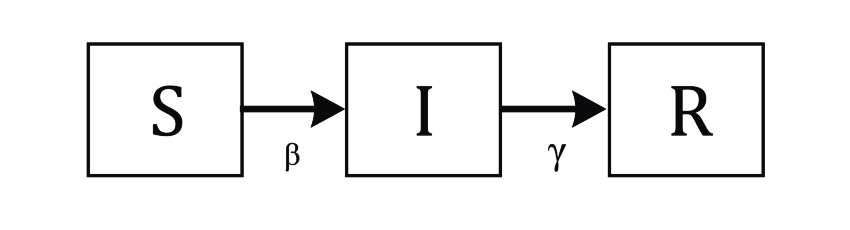
\includegraphics[width=0.8\columnwidth]{SIR-model-flowchart.png} 
	\caption[SIR Gruppenverteilung,\newline Angepasst von https://www.researchgate.net/figure/SIR-model-flowchart\textunderscore fig8\textunderscore 318394911]{SIR Gruppenverteilung}
	\end{figure}

%------------------------------------------------

\subsection{Anwendung}

Das \textbf{SIR-Modell} in der hier dargestellten Form kann das Verhalten einer Epidemie anhand zwei unveränderlicher Parameter darstellen und zeigt so auf wie lange es braucht, bis eine Bevölkerungsgruppe die Infektion überstanden hat. Auch die Menge an Personen, welche bis zum Ende in der suszeptiblen Gruppe (\textit{S}) verblieben sind kann ermittelt werden. 
Begrenzt wird das Modell durch die Tatsache, dass es durch den einfachen Aufbau mit wenigen Parametern und unrealistischen Voraussetzungen nur einen ungefähren Verlauf, jedoch keine exakte und detaillierte Auskunft über Realszenarien bietet.
Durch die Annahme das zu Beginn keine Immunität existiert, und die Parameter als konstant betrachtet werden ist das Modell des Weiteren nicht zur Berechnung von Infektionswellen, sondern nur zur Darstellung eines einmaligen Ausbruchs geeignet.
Allerdings bildet das \textbf{SIR-Modell} eine Grundlage für komplexere Modelle. Diese können für Infektionen/ Umstände angepasst werden, und somit detailreiche Prognosen und Berichte über die Entwicklung einer Epidemie bereitstellen.
So wird beispielsweise in \textsl{"'The SIR Model with Vital Dynamics"'} \cite{5} durch das Hinzufügen von Parametern für Geburten und Todesfälle die Gesamtbevölkerung als Dynamisch betrachtet um sich einem Realbeispiel anzunähern.
Zusätzlich können die Populationsgruppen erweitert oder verringert werden, dies führt dann zu Modellen wie dem 
\textbf{SIRS-Modell}, das eine erneute Infektion ermöglicht und somit auch für Infektionswellen genutzt werden kann, dem \textbf{SEIR-Modell}, bei dem die Personengruppe der Exponierten \textit{E} 
(engl. Exposed)  hinzugefügt wird die infiziert wurde, jedoch noch nicht ansteckend ist oder dem \textbf{SI-Modell}, in welchem Individuen keine Immunität aufbauen.
Einige dieser Modelle werden in \textsl{3.4} genauer beschrieben.
Ein weiterer Anwendungsgrund des Modells ist die Bestimmung der Basisreproduktionszahl (siehe \textsl{3.2}), welche angibt, ob sich eine Infektion zu einer Epidemie entwickelt, sich endemisch hält oder auf Dauer ausstirbt \cite{2}.
So ist das Modell als solches zwar nur als ein mathematisches Idealverhältnis einer Epidemie von Nutzen, doch ist es ein essenzieller Teil der modernen Infektionsepidemiologie und wird von Forschen auf der ganzen Welt dafür genutzt, virale Krankheiten zu dokumentieren und den Ausbruch in eine Epidemie zu verhindern \cite{3}.
%----------------------------------------------------------------------------------------

\section{Mathematischer Aufbau}

Da nun die wichtigsten Begriffe und Bedingungen für das \textbf{SIR-Modell} nun bekannt sind widmet sich dieses Kapitel der Funktion und Zusammensetzung des Modells auf mathematischer Ebene. Danach wird der Fokus auf die Basisreproduktionszahl sowie auf einige Abweichungen des Modells gelegt. Auch die grafische Darstellung des Modells wird angesprochen.
Wenn eine konstante Bevölkerung \textit{N} in drei Gruppen aufgeteilt wird, kann \textit{N} jetzt zu jedem Zeitpunkt (\textit{t}) folgendermaßen definiert werden \cite{3,4}:

$$ \large\textit{S}_{(t)} + \textit{I}_{(t)} + \textit{R}_{(t)} = \textit{N}\normalsize $$

Oder proportional wobei die Werte der Populationen zwischen 0 und 1 liegen. 1 ist hier als 100\%, und 0 als 0\% der gesamten Bevölkerung zu interpretieren:

$$ \large\textit{S} + \textit{I} + \textit{R} = 1 $$

Während die das Modell definierenden Parameter \textbeta\space und \textgamma\space konstant sind, verändern sich die Größen \textit{S}, \textit{I} und \textit{R} im Verlauf von \textit{t}. Man spricht von einem "`Geschlossenen System"' \cite{4}.

%------------------------------------------------

\subsection{Variablen des SIR Modells}

Das \textbf{SIR-Modell} lässt sich durch ein System gewöhnlicher Differentialgleichungen beschreiben.
Dazu werden zunächst die konstanten Parameter noch einmal genauer betrachtet: Die Erholungsrate \textgamma\space beeinflusst, wie lange die Infektion durchschnittlich anhält und wird folgendermaßen berechnet:

$$ \gamma = \frac{1}{T} $$

Wenn also \textit{T} drei Tagen entspricht, ist \textgamma\space ein Drittel. Die Übertragungsrate \textbeta\space hingegen beschreibt, wie oft eine Begegnung der Gruppen \textit{S} und \textit{I} vorkommt, die zu einer Infektion des Individuums der \textit{S} Population führt \cite{2}. 
Im klassischen \textbf{SIR-Modell} wird davon von einer vollkommenen Zufälligkeit der Kontakte ausgegangen. Der Parameter kann durch Faktoren wie Hygiene beeinflusst werden \cite{2,7}.
Da das Modell die Veränderung nur in eine Richtung zulässt (\textit{S} \textrightarrow\space \textit{I} \textrightarrow\space \textit{R}) lässt sich feststellen das die Menge \textit{S} nur abnehmen, und die Menge \textit{R} nur zunehmen kann, und beide von \textit{I} beeinflusst werden.\\
Anhand dieser Informationen lassen sich folgende nichtlineare Differenzialgleichungen für die Änderungsraten, also die Populations-Größenveränderung, zu dem Zeitpunkt \textit{t} aufstellen:

$$ \frac{\Delta S}{\Delta t} = -\beta\space S I $$
\begin{center}
\textsl{Änderungsrate der suszeptiblen Population s'(\textit{t})}
\end{center}

Die suszeptible und die infizierte Population haben den Parameter \textbeta \space gemeinsam. \textit{S} wird mit der Rate \textbeta \space eine Menge an Individuen abgezogen (-\textbeta) und dann \textit{I} hinzugefügt. Da \textit{I} aus mehreren infizierten Individuen besteht, welche jeweils \textbeta\space viele Suszeptible anstecken können, wird \textbeta\textit{S} mit \textit{I} multipliziert.
Die Population der entfernten Individuen wird berechnet indem der Parameter \textgamma\space mit \textit{I} malgenommen wird, da \textit{I} mit der Rate \textgamma\space entfernt wird \cite{7,3}:

$$ \frac{\Delta R}{\Delta t} = \gamma I $$
\begin{center}
\textsl{Änderungsrate der entfernten Population r'(\textit{t})}
\end{center}


Da alle Gleichungen zu jedem Zeitpunkt zusammen 1 ergeben müssen (\textit{S} + \textit{I} + \textit{R} = 1) und \textit{I} ein Faktor der anderen Gleichungen ist, kann s'(\textit{t}) durch Kombination der anderen Gleichung und Umkehrung der Parameter bestimmt werden
 \cite{3, 4}:

$$ \frac{\Delta I}{\Delta t} = \beta\space S I - \gamma I $$
\begin{center}
\textsl{Änderungsrate der infizierten Population s'(\textit{t})}
\end{center}

Hier bekommt \textit{I} Zuwachs von \textit{S} mit dem Parameter \textbeta\space und nimmt mit dem Parameter \textgamma\space ab.

%------------------------------------------------

\subsection{Reproduktionsrate einer Infektion}

Wenn eine aktuelle Infektion mit dem \textbf{SIR-Modell} betrachtet wird, soll an erster Stelle erkenntlich gemacht werden wie sich die Infektion verhält oder einwickeln wird. Es gibt drei Verhaltensweisen, die durch das \textbf{SIR-Modell} festgestellt werden können:\\

\begin{itemize}
	\item \textbf{Endemisch} wird eine Infektion benannt, die regelmäßig lokal auftritt und einigermaßen konstante Infektionen aufweist.\\
	
  \item \textbf{Epidemisch} wird eine Infektion dann genannt, wenn an einem Ort schneller Neuinfektionen auftreten wie bereits Infizierte genesen/sterben, sie sich also verbreitet.
\end{itemize}

Eine globale Epidemie wird als Pandemie bezeichnet und nicht separat von dem \textbf{SIR-Modell} erfasst. Das epidemische Verhalten wird in zwei Phasen aufgeteilt: Ausbreitung und Rückgang. Als Folge davon, dass nach einer gewissen Zeit die meisten oder alle Individuen in die infizierte oder entfernte Population aufgerückt sind, sind Neuinfektionen nicht mehr oder nur schwer möglich, sodass die Infektionswelle abflacht \cite{3,5}. Das \textbf{SIR-Modell} ermöglicht die Berechnung der sogenannten Basisreproduktionszahl  $r_{0}$
welche zu Beginn der Infektion t = 0 das zukünftige Verhalten der Krankheit angibt. Berechnet wird diese anhand der beiden Parameter \textbeta\space und \textgamma\space welche die Zu- und Abnahme der Population \textit{I} beschreiben. Des Weiteren spielt auch die proportionale Größe von \textit{S} eine Rolle, da zur Infektion ein suszeptibles Individuum benötigt wird. Zu Beginn des Modells beträgt \textit{S} ungefähr 1, und kann daher bei der Berechnung der Basisreproduktionszahl vernachlässigt werden. Deshalb gilt solange die Übertragungsrate \textbeta\space größer als die Erholungsrate \textgamma\space ist nimmt die Menge der Population \textit{I} zu. Die Rechnung dazu sieht folgendermaßen aus \cite{6,3}:

$$ r_{0} = \frac{\beta}{\gamma} $$

\begin{center}
\textit{r_{0} > 1 =} \textnormal{Epidemisch}, r_{0} \approx 1 = \textnormal{Endemisch}, r_{0} < 1 = \textnormal{Rückgängig.}
\end{center}\\
Im Fall von R = 2, infiziert jedes Individuum der Population \textit{I} zwei weitere Personen, bevor es in \textit{R} übergeht. In diesem Fall wird von exponentiellem Wachstum gesprochen.
Wenn man die derzeitige Reproduktionszahl eines Zeitpunkts \textit{t} ermitteln möchte, um herauszufinden in welchem Zustand sich die Infektion befindet, muss die Änderungsrate von \textit{S} berücksichtigt werden:

$$ r_{t} = \frac{\beta S_{t}}{\gamma} $$

Mithilfe dieser Gleichung lässt sich beispielsweise erkennen, welchen Effekt getroffene Maßnahmen (Social Distancing, Impfung, Ausgangsbeschränkungen, Schulschließungen etc.) auf die Ausbreitung der Infektion haben 
(siehe 3.5).

%------------------------------------------------

\subsection{Grafische Darstellung des SIR-Modells}

Ein essenzieller Part des \textbf{SIR-Modells} ist die grafische Darstellung des Infektionsverlaufs um eine Übersicht der Epidemie für die Allgemeinheit zu visualisieren, und das schnelle Auslesen von Daten an spezifischen Punkten zu ermöglichen.
In einem Koordinatensystem stellt die x-Achse die Zeit in Tagen, und die y-Achse die Bevölkerungsanzahl dar. Drei Graphen der in 3.1 angesprochenen Gleichungen zeigen die Änderung der Größe der jeweiligen Population auf.\\
\\
Auch hier gilt das zu jedem Zeitpunkt die Summe der Flächen unter den Graphen die Größe \textit{N} ergibt welche so eine horizontale Asymptote für die Graphen bildet (Abb. 3.1).
Die Startwerte der Gruppen an t = 0 sind: 
$S_{0} \approx 1, I_{0} \approx 0$ wobei: $ S_{0} < 1, I_{0} > 0$ sodass beide zusammen die Menge 1 ergeben \cite{4},
weil zu Beginn kein Individuum Immunität besitzt und sich mindestens eine infizierte Person in der Bevölkerung befinden muss, um den Ausbruch auszulösen. Daher gilt: $R_{0} = 0, R_{0} \geq 0$ (nicht zu verwechseln mit der Basisreproduktionszahl $r_{0}$).
In dieser Grafik (Abb. 3.1) lässt sich auslesen dass das Wachstum der Epidemie an Tag 20 endet, da der Graph von \textit{I} an dieser Stelle einen Hochpunkt hat. Auch wann sie ausstirbt (ungefähr Tag 70) sowie die Menge der Individuen die zu keinem Zeitpunkt infiziert waren (0) können abgeleitet werden \cite{1}.

	\begin{figure}[h]
	\centering
	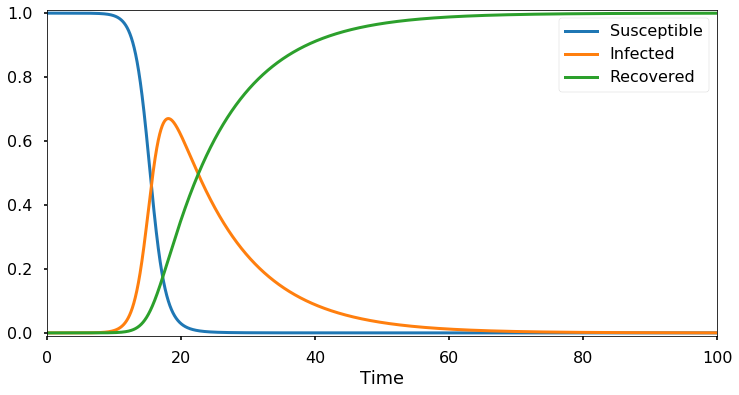
\includegraphics[width=0.8\columnwidth]{SIR-model-graph.png}
	\caption[SIR Infektionsverlauf,\newline https://www.davidketcheson.info/2020/03/17/SIR\textunderscore model.html]{SIR Infektionsverlauf}
	\end{figure}

%------------------------------------------------

%\subsection{Berechnung der Maximalen Anzahl von \textit{I}}

%Der Moment an dem eine Infektion die Meisten Individuen zur selben Zeit infiziert hat kann als Wendepunkt der Epidemie gesehen werden und findet zu dem Zeitpunkt statt, in welchem die Effektive Reproduktionsrate \textit{r} = 1 beträgt. Diese sinkt von beginn der Pandemie an, da durch steigende Infektionen die Suszeptiblen in die Infizierte Population übergehen und so weniger Kontakte mit beiden Gruppen entstehen. Die Menge an Individuen, welche über den gesamten verlauf Maximal gleichzeitig Infiziert werden können ist eine wichtige Information für die Verteilung von Gesundheitsressourcen wie Masken, Krankenhausbetten oder Impfungen und somit ein essenzieller faktor zur Eindämmung der Epidemie. Um den wert von $\textit{S}_{max}$ Herauszufinden, wird zunächst die änderungsrate von \textit{I} durch die Änderungsrate von \textit{S} gerechnet, was folgendermaßen vereinfacht werden kann:

%$$ \frac{\Delta I}{\Delta S} = \frac{\beta I S - \gamma I}{-\beta I S} = -1 + \frac{\gamma}{\beta S}$$




%$$ \frac{\Delta I}{\Delta S} = -1 + \frac{1}{r S}$$

%$$ I_{max} = I_{0} + S_{0} - \frac{1}{r} $$

%Auch wenn die Graphische Darstellung ein ungefähres Ablesen der Werte zu jedem Zeitpunkt ermöglicht, können Wichtige Ereignisse wie dem Punkt an dem \textit{I} den größten wert hat durch eigene Gleichungen Berechnet werden. Bei einem Infektionsverlauf des \textbf{SIR-Modells} steigt die Anzahl der Infizierten so lange an, bis die Reproduktionsrate 1 erreicht.

%------------------------------------------------

\subsection{Variationen des SIR-Modells}

Nachdem die grundlegenden Rechnungen und Parameter des \textbf{SIR-Modells} nun bekannt sind, werden im Folgenden einige gängige Variationen des Modells genauer betrachtet. Wie bereits erwähnt ist das Modell prädestiniert dafür, verändert oder erweitert zu werden um exaktere Berechnungen an Epidemien zu ermöglichen. Diese Veränderungen können das Hinzufügen weiterer Populationen, Parameter, sowie das Anpassen der Startbedingungen beinhalten \cite{5}.

%---------------------

\subsubsection{Modell zur Berechnung von Infektionswellen}

Wie am Beispiel \textsl{Covid-19} zu erkennen ist, gibt es Epidemien die keine oder nur temporäre Immunität erlauben. Dies bedeutet das Infektionswellen entstehen, in welchen die Infektion ausbricht und wieder zurückgeht. Um das \textbf{SIR-Modell} für eine solche Situation anzupassen, kann entweder die entfernte Gruppe durch eine Suszeptible ersetzt werden, welches \textbf{SIS-Modell} genannt wird, oder eine weitere suszeptible Gruppe zu einem \textbf{SIRS-Modell} angefügt werden. Die Startbedingungen und Parameter für das \textbf{SIS-Modell} bleiben identisch zu dem \textbf{SIR-Modell}.\\
Aus den drei Differentialgleichungen werden zwei:

$$ \frac{\Delta S}{\Delta t} = -\beta\space S I + \gamma I $$
$$ \frac{\Delta I}{\Delta t} = \beta\space S I - \gamma I$$

\textit{S} nimmt mit \textbeta\space ab, bekommt jedoch die Menge \textgamma\space dazu, während für \textit{I} das genaue Gegenteil gilt. Individuen bewegen sich so von \textit{S} zu \textit{I} in einem ewigen Kreislauf
\cite{5}.
Das \textbf{SIRS-Modell} wird eingesetzt, wenn eine nur temporäre Immunität besteht, wie es bei \textsl{Covid-19} der Fall ist. Diese Variation des Modells führt den Parameter Epsilon (\textepsilon)\space als durchschnittliche Immunitätsdauer ein. Hier werden die Änderungsraten angepasst indem Individuen von \textit{R} mit der Rate \textepsilon\space zu \textit{S} übergehen, was erneut in einem Kreislaufmodell endet \cite{8}:

$$ \frac{\Delta S}{\Delta t} = -\beta\space S I + \epsilon R $$
$$ \frac{\Delta I}{\Delta t} = \beta\space S I + -\gamma I $$
$$ \frac{\Delta T}{\Delta t} = \gamma I - \epsilon R $$\\

%---------------------
\subsubsection{Modell mit dynamischer Gesamtbevölkerung}

In der Realität gibt es viele Faktoren, die die Bevölkerung nicht konstant halten. Das \textbf{SIR-Modell} mit \textbf{Dynamischer Bevölkerung} versucht durch die erweiterten Parameter Nu (\textnu)\space für Geburten und Mu (\textmu)\space für Todesfälle einige der wichtigsten Faktoren einer dynamischen Bevölkerung miteinzubeziehen. Neugeburten werden in die suszeptible Population eingeordnet, während Tode in jeder Population präsent sind. Dementsprechend werden diese Parameter zu den Änderungsraten hinzugefügt oder abgezogen \cite{8}:

$$ \frac{\Delta S}{\Delta t} = -\beta\space S I + \nu - \mu S $$
$$ \frac{\Delta I}{\Delta t} = \beta\space S I -\gamma\space I - \mu I $$
$$ \frac{\Delta R}{\Delta t} = \gamma\space I - \mu R $$

Diese Anpassung findet Anwendung in den meisten Modellen, die eine Epidemie über einen längeren Zeitraum hin betrachten, da die Abweichung der Menge der Gesamtbevölkerung auf Dauer zu groß wird um ignoriert zu werden.

%------------------------------------------------

\subsection{Berechenbare Werte des SIR-Modells}

Es gibt eine Menge wertvoller Daten, die durch den Gebrauch des \textbf{SIR-Modells} oder dessen Derivate errechnet werden können.
Wenn in einer Bevölkerung eine gewisse Anzahl an Personen Immunität gegen eine Infektion aufweist, kann sich die Epidemie nicht länger verbreiten, obwohl \textsl{S} noch Individuen beinhaltet. Dieses Phänomen wird Herdenimmunität oder Herdenschutz genannt. Sie kann durch die Epidemie selbst auftreten, wenn ein Großteil der Bevölkerung durch einmalige Infektion immunisiert wird, oder durch Impfungen beschleunigt werden \cite{3}.\\
Die Bedeutung dieses Schwellenwerts hat sich während des Ausbruchs von \textsl{Covid-19} gezeigt. Es wurde versucht, möglichst schnell durch Impfungen die Herdenimmunität zu erreichen \cite{10}. Anhand des \textbf{SIR-Modells} lässt sich berechnen, wann die Epidemie selbst den Herdenschutz auslöst, in dem der Zeitpunkt von $ \textit{I}_{max} $ bestimmt wird. Auch die Menge von $ \textit{I}_{max} $ lässt sich errechnen, was aufgrund der Komplexität der Formeln in dieser Arbeit nicht behandelt wird. Einfacher zu ermitteln hingegen ist die Größe von $ \textit{S}_{0} $ damit sich keine Epidemie ausbreiten kann, da sie einen Einfluss auf die Basisreproduktionszahl hat, welche wiederum über das Verhalten einer Infektion entscheidet. 
Dazu muss nur beachtet werden das in diesem Fall bei der Berechnung der Basisreproduktionszahl $\textit{r}_{0} $ die Startmenge von $ \textit{S}_{0}$ nicht vernachlässigt werden darf, da sie nicht der ungefähren Gesamtbevölkerung entspricht \cite{7, 10}:

$$ r_{o} = \frac{\beta S_{0}}{\gamma} $$

Weitere erfassbare Werte beinhalten die Menge der suszeptiblen Population nach Ende der Epidemie sowie die Menge der meisten Neuinfektionen an einem Tag (Auch diese werden in der Arbeit nicht weiter ausgeführt). Eine der nützlichsten Funktionen des \textbf{SIR-Modells} ist die Evaluierung der Auswirkung von Gegenmaßnahmen und Ereignissen wie Mutationen auf den Verlauf der Epidemie. Dies ist essenziell um die Effektivität von einzelnen Maßnahmen in Erfahrung zu bringen. Meistens wird das erreicht, indem die Übertragungsrate \textbeta\space verändert wird, da diese alle Faktoren der Übertragungs- und Infektionswahrscheinlichkeit beinhaltet \cite{8, 6, 9}.

%------------------------------------------------

%\section{Mathematisches Chaos des SIR-Modells}

%In der Mathematik, Chaos 

%leicht veränderte startwerte, starke abweichung (100% social d vs. 90% social d)

%\section{Einflussfaktoren von Infektionen}

%Es gibt eine Menge  \textbf{SIR-Modell} 

%impfung, distancing, Hygiene, Mutationen, herden immunität, superspreader

%----------------------------------------------------------------------------------------

\section{Das SIR-Modell in Anwendung}

Mit dem Verständnis des grundsätzlichen mathematischen Aufbaus des \textbf{SIR-Modells} wird nun der Fall \textsl{Covid-19} genauer analysiert, und mit der saisonalen \textsl{Influenza}-Infektion verglichen. Hiermit soll demonstriert werden, wie flexibel und exakt das Modell in Realszenarien erscheint, und welche Unterscheidungen zwischen verschiedenen Epidemien bestehen. Auch die praktische Anwendung und Funktion von Vorhersagen soll erläutert werden.

%------------------------------------------------

\subsection{"`Coronavirus Disease 2019"'}

Da die \textsl{Covid-19} Pandemie sich derzeitig dem Ende nähert, und die gesamte Welt betroffen ist, gibt es eine Menge Daten, die sich mit getroffenen Vorhersagen des \textbf{SIR-Modells} vergleichen lassen.
Vorhersagen des Modells werden vor allem zur Findung und Überprüfung geeigneter Maßnahmen genutzt, um die Menge an gleichzeitig infizierten Individuen mit schweren Verläufen zu verringern. Mit dem Ziel die Überlastung der Krankenhäuser zu verhindern.\\
Damit das Modell näherungsweise präzise Werte liefert, wird die Gesamtbevölkerung aufgeteilt, sodass nur ein Land oder eine Stadt betrachtet wird. Das ist notwendig da die Erfassung von \textbeta\space und \textgamma\space von vielen lokalen Umständen wie der Temperatur, dem Wetter, der Bevölkerungsdichte und nicht zuletzt den Maßnahmen zur Einschränkung des Virus beeinflusst wird. 
Des Weiteren weist \textsl{Covid-19} eine Inkubationszeit auf, also einen Zeitraum in dem ein Individuum infiziert, jedoch nicht ansteckend ist. Aufgrund dessen wird eine weitere Population \textit{E} zwischen den Suszeptiblen und den Infizierten eingeführt (\textbf{SEIR-Modell}) \cite{11, 3}. Um die durchschnittliche Inkubationsdauer zwischen \textit{S} -> \textit{E} -> \textit{I} zu beschreiben wird der Parameter Alpha (\textalpha)\space verwendet, sodass alle suszeptiblen Individuen zuerst zu \textit{E} übergehen, und dort die durchschnittliche Inkubationszeit verweilen. Die Gleichungen der Änderungsraten werden dementsprechend angepasst \cite{2, 3}:

$$ \frac{\Delta S}{\Delta t} = -\beta S I $$
$$ \frac{\Delta E}{\Delta t} = \beta S I - \alpha E$$
$$ \frac{\Delta I}{\Delta t} = \alpha E - \gamma I $$
$$ \frac{\Delta R}{\Delta t} = -\gamma I $$

Da bei \textsl{Covid-19} die Immunität des Virus nach einer überstandenen Infektion nur für einen gewissen Zeitpunkt gegeben ist, wird der Parameter \textepsilon\space des in 3.4.1 angesprochenen \textbf{SIRS-Modells} in das \textsl{"`Covid-19 Modell"'} eingefügt. Es wird dadurch als \textbf{SEIRS-Modell} betitelt und die Änderungsraten von \textsl{S} und \textit{R} verändern sich folgendermaßen \cite{8}:

$$ \frac{\Delta S}{\Delta t} = -\beta S I + \epsilon R$$
$$ \frac{\Delta R}{\Delta t} = -\gamma I - \epsilon R$$

Dieser Faktor der erneuten Infizierung lässt wellenartige Infektionsausbrüche zu \cite{3}. Bei \textsl{Covid-19} sind bis heute bereits fünf Wellen aufgetreten. Da das \textbf{SIR-Modell} am Besten in kürzeren Zeitabständen funktioniert, wird hier nur die erste Infektionswelle, ohne Impfungen betrachtet.\\
\\
Das Modell, wird hier anhand Abb. 4.1, durch die Anzahl der \textsl{Covid-19} Patienten in Südkorea über einen Zeitraum von 60 Tagen mit real erhobenen Daten verglichen.
Die Menge der Patienten ist der durchschnittliche Teil der Population \textit{I} mit schweren Verläufen, der durch Realdaten erhoben wird \cite{3}. Dabei ist eine starke Ähnlichkeit der beiden Graphen zu erkennen.

	\begin{figure}[h]
	\centering
	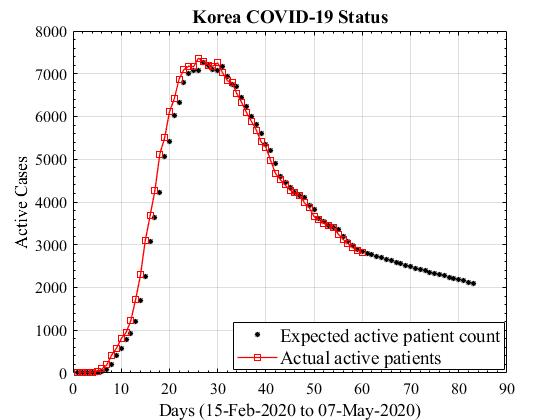
\includegraphics[width=0.65\columnwidth]{Covid-korea-chart.jpg}
	\caption[Infektionskurve von Südkorea,\newline https://cmte.ieee.org/futuredirections/tech-policy-ethics/may-2020/covid-19-disease-modelling-and-its-impact-on-public-health-policy/]{Infektionskurve von Südkorea}
	\end{figure}
	
Das Modell kann wie gezeigt trotz des vergleichbar einfachen Aufbaus, gute Vorhersagen zu simplen epidemischen Ausbrüchen treffen.
Damit kann nun durch absichtliches Manipulieren der Parameter auch eine Vorhersage zu eventuellen Mutationen oder Gegenmaßnamen getroffen werden. Im Beispiel eines Lockdowns wird die Kontaktwahrscheinlichkeit der Populationen \textit{S} und \textit{I} um einen errechneten Wert verringert, mit der Folge das der Parameter \textbeta\space und somit die Reproduktionsrate \textit{r} sinkt. In Abb. 4.2 ist eine solche Maßnahme für die indische Stadt Rajasthan errechnet, und getroffen worden. In der Grafik stellt Orange die normale errechnete Infektionsrate, Blau die errechnete Infektionsrate mit angewandtem Lockdown und Lila die Echtdaten mit Lockdown dar \cite{3, 10, 11}. Die errechnete Lockdown-Kurve weist erneut eine große Ähnlichkeit mit den Echtdaten auf.
Daraus lässt sich ableiten, wie präzise die Abwandlung des \textbf{SIR-Modells} die Realität widerspiegelt, und als geeignete Methode angewendet werden kann.
	
	\begin{figure}[h]
	\centering
	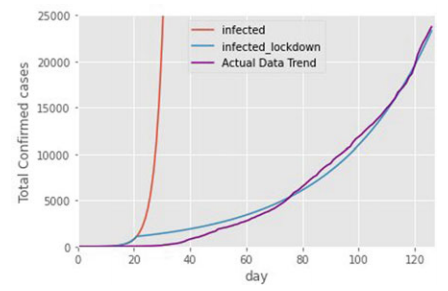
\includegraphics[width=0.7\columnwidth]{SIR-data-trend.png}
	\caption[Infektionskurve mit Lockdown in Rajasthan,\newline Entnommen aus: \cite{3}]{Infektionskurve mit Lockdown in Rajasthan}
	\end{figure}
	
Wie an Tag 20 allerdings zu erkennen ist, gibt es einige unvorhersehbare Faktoren wie \textsl{"`Superspreader"'}, Personen die eine wesentlich größere Menge als den Durchschnitt an suszeptiblen Individuen infizieren, oder wie in dem Fall der Abbildung 4.2 das plötzliche Wachstum von \textsl{S} durch die Rückkehr von Reisenden aufgrund des ausgerufenen Lockdowns \cite{3, 11}.

%------------------------------------------------
\newpage
\subsection{Vergleich mit Influenza}

\textsl{Influenza} ist eine "`Virale Infektionskrankheit"' mit starker Ähnlichkeit zu \textsl{Covid-19} in der Infizierung mittels Aerosolen und Husten. Der bekannteste Ausbruch fand 1918-1920 durch die Spanische Grippe statt, bei der etwa 500 Millionen Menschen infiziert wurden und circa 20 Millionen starben. \textsl{Influenza} mutiert häufig und tritt so alljährlich epidemisch auf \cite{2, 3}. Der Grund das \textit{Influenza} trotz vergleichbarer Verbreitung zu \textsl{Covid-19} nicht dieselbe Auswirkung in der Welt hat ist die verglichen geringe Übertragungsrate. Während \textsl{Covid-19} eine Reproduktionsrate von bis zu 6.0 aufweist, hat die Saisonale \textsl{Influenza-Grippe} ein Maximalwert von circa 2.8, an manchen Orten wesentlich weniger. Ein weiterer Faktor ist die Impfung, welche vulnerablen Gruppen Schutz durch Immunität gewährt. Das trägt dazu bei, das weniger schwere Verläufe gleichzeitig auftreten, und die Verbleibenden sofort behandelt werden können \cite{3}. Dennoch versterben laut der WHO jährlich zwischen 290.000 und 650.000 Menschen, größtenteils in Entwicklungsländern an dem Virus. Zur Berechnung von \textsl{Influenza} wird das \textbf{SEIR-Modell} angewandt, da eine Inkubationsphase vorliegt, und Individuen nach der Infektion immun gegen das Virus sind. Das gilt jedoch nicht unbedingt für Mutationen. Durch die häufigen Mutationen ist es relativ kompliziert, die Infektion vorherzusagen \cite{11}.


%----------------------------------------------------------------------------------------
\newpage
\section{Fazit}

In dieser Arbeit wurden die Berechnung und Visualisierung von Infektionen mit epidemischem Verhalten und den vorausgesetzten Bedingungen der Verbreitung in einer Population über einen Zeitraum durch die Verwendung des \textbf{SIR-Modells} behandelt. Das Aufteilen der Gesamtbevölkerung \textit{N} in die suszeptible, infizierte und entfernte Gruppe und ihre jeweilige Bedeutung wurde mit allen Zusammenhängen erklärt. Ebenso wurden alle Bedingungen und Einschränkungen des Modells ausführlich aufgezeigt.
Die Parameter \textbeta\space als Rate der Infektion, die sich aus der durchschnittlichen Kontakt- und Übertragungswahrscheinlichkeit zwischen den Gruppen \textit{S} und \textit{I} zusammensetzt, sowie die Erholungsrate \textgamma\space, der durchschnittlichen Dauer der Infektion, wurden mit ihrem Einfluss auf den Verlauf der Epidemie beschrieben. Mithilfe der Populationen und Parametern wurden die drei grundlegenden Differenzialgleichungen des Modells aufgestellt und beschrieben. Anhand dessen wurde eine Möglichkeit der Visualisierung in Form eines Koordinatensystems und den Graphen der Gleichungen aufgezeigt.
Verschiedene Varianten des \textbf{SIR-Modells} wurden angesprochen, die die Kalkulation von weiteren Infektionen ermöglichen, und die Präzision der Rechnungen für einige Epidemien erhöhen. Durch den Einsatz des \textbf{SIR-Modells} an der \textsl{Covid-19} Pandemie konnte festgestellt werden, dass das Modell, im Anbetracht eines kurzen Zeitabschnitts und einer kleinen Bevölkerung durchaus genaue Werte liefern kann. Es eignet sich jedoch nicht für eine Erfassung der gesamten Weltbevölkerung durch die Vielzahl an unerwarteten Ereignissen und Unterschieden. Durch den Vergleich mit der \textsl{Influenza}-Infektion wurde die vielseitige Anwendung des Modells, sowie die Unterschiede und Gemeinsamkeiten zwischen Epidemien verdeutlicht.\\
\\
Das \textbf{SIR-Modell} liefert trotz seines simplen Aufbaus dennoch ungefähre bis genaue Werte über eine Epidemie und ist deshalb eine exzellente Wahl um schnell und einfach einen Überblick von Informationen über eine Infektion zu erhalten, und die Effektivität von Gegenmaßnamen in Erfahrung zu bringen.

%----------------------------------------------------------------------------------------

\newpage
\setlength{\bibitemsep}{\baselineskip}
\printbibliography[heading=bibintoc]
\thispagestyle{empty}
\newpage
\cleardoublepage
\listoffigures
\thispagestyle{empty}

\newpage
\section*{Eidesstattliche Erklärung}
\thispagestyle{empty}
\vfill
„Ich versichere, dass ich diese Seminararbeit ohne fremde Hilfe angefertigt und nur die angegebenen Quellen und Hilfsmittel benützt habe.“\\
\\
\\
\\
.............................., den ............................ \hfill .....................................\\
\begin{flushright}
Unterschrift
\end{flushright}

\end{document}
